% Provenance (never printed): see sources/outline_sources.md (Year 3:
% energy-balance models, the one-layer model recalled; ice-albedo feedback
% and multiple equilibria; how general circulation models are built and
% evaluated).
% Brief: sources/book5/BRIEFS.md, ch. 22. Curves from
% figdata/bachelor-3/budyko_sellers.py (the zero-dimensional model and
% Budyko's latitudinal model; the brief's ebm_0d is folded into it) and
% two_layer.py. Exercise and problem values in the Book 5 scratch calculator
% calc/ch22.py. The model planet, model X and the ensemble of exercise 12 are
% invented.
\chapter{نماذج المناخ}\label{ch:b3:climate-models}

لنأخذ ضوء الشمس الواصل إلى الأرض، \qty{340}{W/m^2} متوسطًا على الكرة
الأرضية، وقانونًا للأشعة تحت الحمراء التي تعيدها إلى الفضاء، مُطابَقًا
لثلاثين سنةً من إعادة تحليل الرصدات. ولنفترض أنّ ألبيدو الكوكب يرتفع من ألبيدو
اليابسة المكشوفة والمحيط إلى ألبيدو الجليد مع برودة السطح. ونوازن الدفقين،
فيكون للمعادلة ثلاثة حلول: كوكب درجة حرارته
\qty{14}{\celsius}، قريبة من متوسط الكوكب الحقيقي؛ وكوكب درجة حرارته
\qty{8}{\celsius}؛ وكوكب درجة حرارته \qty{-46}{\celsius}، متجمّد من القطب إلى
القطب. النماذج المناخية، من هذه الأسطر القليلة إلى البرامج التي تُشغَّل على أكبر
الحواسيب، أدوات لطرح سؤال أيّ مناخ يملكه كوكب معيّن، وكيف يصل إليه،
وكيف يتغيّر حين يختلّ توازن طاقته.
% ledger: nasa:solar-mean, data:b5-ncep-air, data:b3-ncep, budyko69:albedo

\begin{recall}
الجسم الأسود، وقانون ستيفان--بولتزمان، وتأثير الاحتباس الحراري، ونموذج الطبقة الواحدة للغلاف الجوي
ترد في كتب الفيزياء؛ والألبيدو
وميزانية طاقة الأرض في الكتب المدرسية. الإشعاع طويل الموجة الخارج
ودرجة حرارة الانبعاث والنقل الحراري الميريدي ترد
في مجلد السنة الأولى، في فصله عن الإشعاع ونقل الحرارة. ويرد
التغذية الراجعة للجليد والألبيدو، والأرض كرة الثلج، ترد في مجلد السنة الثانية، في
فصله عن الأرض في ما قبل الكمبري؛ والتأثير الإشعاعي الفعّال،
وبارامتر التغذية الراجعة المناخية $\lambda < 0$، والحساسية المناخية عند التوازن
\babelsublr{(ECS)} والاستجابة المناخية العابرة \babelsublr{(TCR)}، في فصله عن
تغيّر المناخ الناجم عن الإنسان؛ والتنبؤ العددي بالطقس،
وتنبؤ المجموعة في فصله عن أنظمة الطقس. وتُعرض معادلات
الحركة على الأرض الدوّارة، مع \omterm{def:b3:gfd-foundations:hydrostatic}{التقريب الهيدروستاتيكي}، ترد في
الفصل~\ref{ch:b3:gfd-foundations}.
\end{recall}

\section{توازن الطاقة في الكوكب}\label{sec:b3:climate-models:zero-d}

متوسطًا على الكرة وعلى مدار السنة، يستقبل كلُّ متر مربّع عند قمّة
الغلاف الجوي $Q = S_0/4 = \qty{340}{W/m^2}$، ربعَ
الإشعاع الشمسي $S_0 = \qty{1360}{W/m^2}$. ويُعكس جزء $\alpha$، وهو الألبيدو
الكوكبي؛ والباقي $Q(1 - \alpha)$ يُمتصّ،
ويجب أن يُعاد إلى الفضاء على هيئة أشعة تحت حمراء. يُصدر الجسم الأسود $\sigma
T^4$؛ والإشعاع طويل الموجة الخارج من الأرض \babelsublr{(OLR)} أصغر بسبب
تأثير الاحتباس الحراري، وعلى مدى درجات حرارة السطح الموجودة على
الأرض فإنّه يقارب خطًّا مستقيمًا،
\[
\text{OLR} = A + BT ,
\]
مع $T$ درجة حرارة السطح بالدرجات المئوية. في عام 1969 طابق بوديكو
هذا القانون على الإشعاع الخارج المحسوب في 260 محطّة، مع تصحيح
لتأثير الغيم $n$: $I = a + bT - (a_1 + b_1T)n$، $a = 14.0$، $b = 0.14$، $a_1 =
3.0$ و$b_1 = 0.10$ بوحدة \unit{kcal.cm^{-2}} لكل شهر، مع تشتّت أقلّ من
\qty{5}{\percent}. ومن أجل متوسط غيم قدره 0.5 يُعطي $A =
\qty{199}{W/m^2}$ و$B = \qty{1.43}{W.m^{-2}.\celsius^{-1}}$. أمّا المتوسطات
النطاقية السنوية \babelsublr{NCEP--NCAR Reanalysis~1} للفترة 1991--2020، موزونةً بالمساحة،
فتعطي $A = \qty{211.9}{W/m^2}$ و$B = \qty{1.816}{W.m^{-2}.\celsius^{-1}}$،
مع تشتّت قدره \qty{10}{W/m^2} حول الخط. تُستعمل هذه القيم
في ما يلي.
% ledger: nasa:solar-mean, budyko69:olr, data:b5-ncep-air, data:b3-ncep

\begin{definition}[نموذج توازن الطاقة]\label{def:b3:climate-models:ebm}
\emph{نموذج توازن الطاقة}\index{نموذج توازن الطاقة} نموذجٌ مناخي
يحسب درجة حرارة السطح --- متوسطًا عالميًّا واحدًا، أو متوسطًا
على كلّ خط عرض --- انطلاقًا من توازن ضوء الشمس الممتص، والأشعة
تحت الحمراء المنبعثة إلى الفضاء، وإن كانت درجة الحرارة تتعلّق بخط العرض،
والحرارة المحمولة نحو القطبين. وفي صيغته ذات البعد الصفري،
\[
C\,\frac{\mathrm dT}{\mathrm dt} = Q\big(1 - \alpha(T)\big) - (A + BT) ,
\]
حيث $C$ هي السعة الحرارية لكل وحدة مساحة من جزء النظام الذي
يتسخّن مع السطح.
\end{definition}

بوضع $\alpha = 0.30$ يكون التوازن $T = (238 - 211.9)/1.816 =
\qty{14.4}{\celsius}$؛ والمتوسط المساحي لإعادة التحليل يساوي
\qty{14.2}{\celsius}. ويُضاف التأثير $F$، مثل تأثير تغيّر ثاني أكسيد الكربون،
إلى الطرف الأيمن. وقرب أحد التوازنات تتحدّد الاستجابة
بدلالة بارامتر التغذية الراجعة المناخية $\lambda$ من مجلد السنة الثانية:
مع ثبات الألبيدو، $\lambda = -B$.
% ledger: earth:albedo, data:b5-ncep-air

\begin{theorem}[زمن الاستجابة لمناخ ذي صندوق واحد]\label{thm:b3:climate-models:response}
ليكن المناخ في توازن، ولنفترض أنّ تأثيرًا ثابتًا $F$ يُفعَّل
عند $t = 0$. فإذا كان الانحراف $T'$ عن التوازن يحقّق $C\,\mathrm
dT'/\mathrm dt = F + \lambda T'$ مع $C > 0$ و$\lambda < 0$ ثابتين،
فإنّ
\[
T'(t) = -\frac{F}{\lambda}\Big(1 - \mathrm e^{-t/\tau}\Big), \qquad
\tau = -\frac{C}{\lambda} .
\]
والتوازن الجديد هو $-F/\lambda$، ويقطع المناخ الكسرَ $1
- \mathrm e^{-1} = \num{0.63}$ من المسافة في الزمن $\tau$.
\end{theorem}

\begin{proof}
$T'_\infty = -F/\lambda$ يجعل الطرف الأيمن يساوي صفرًا. والفرق
$u = T' - T'_\infty$ يحقّق $C\,\mathrm du/\mathrm dt = \lambda u$، فإنّ $u =
u(0)\,\mathrm e^{\lambda t/C}$، مع $u(0) = F/\lambda$.
\end{proof}

السعة الحرارية المؤثّرة خلال بضع سنوات هي سعة المحيط العلوي.
المحاكي ذو الطبقتين للتقرير السادس للتقييم الصادر عن الهيئة
الحكومية الدولية المعنيّة بتغيّر المناخ، المعايَر على 44 نموذجًا مناخيًّا،
يعطي طبقة السطح $C = \qty{8.1}{W.yr.m^{-2}.\celsius^{-1}}$، أي السعة الحرارية
لطبقة من مياه البحر عمقها \qty{62}{m}. ومع $\lambda = -B$ فإنّ
زمن الاستجابة هو $8.1/1.816 = \num{4.5}\text{ سنة}$. ويُسخّن المناخ الحقيقي أيضًا
المحيط العميق، ببطء أكبر بكثير؛ والقسم~\ref{sec:b3:climate-models:two-layer}
يُدرجه.
% ledger: ar6sm7:two-layer, teos10:cp0, data:b5-ncep-air

\section{الجليد والألبيدو والتوازنات المتعدّدة}\label{sec:b3:climate-models:multiple}

تجعل تغذية الجليد والألبيدو الراجعة الواردة في مجلد السنة الثانية الألبيدوَ يعتمد على
درجة الحرارة. نأخذ $\alpha = 0.62$ لكوكب يقع سطحه أدنى من
$T_I = \qty{-10}{\celsius}$، وهو ألبيدو الجليد في نموذج بوديكو، $\alpha
= 0.30$ فوق $T_F = \qty{+10}{\celsius}$، وخطًّا مستقيمًا بينهما، مع تراجع الجليد.
المنحدر اختيارٌ خاصّ بهذا الفصل؛ وأيّ ألبيدو يرتفع
مع برودة الكوكب يعطي الصورة ذاتها.
% ledger: budyko69:albedo, earth:albedo

\begin{definition}[التوازنات المناخية المتعدّدة؛ التشعّب السرجي العقدي]\label{def:b3:climate-models:multiple-equilibria}
يكون للنموذج المناخي \emph{التوازنات المناخية المتعدّدة}\index{التوازنات المناخية المتعدّدة}
حين يملك، عند الشروط الخارجية نفسها، أكثر من
حالة مستقرّة واحدة. يكون التوازن مستقرًّا إذا تلاشى انحراف صغير عنه،
ويكون غير مستقرّ إذا نما. \emph{التشعّب السرجي
العقدي}\index{التشعّب السرجي العقدي} هو قيمة الوسيط التي
يلتقي عندها توازن مستقرّ وتوازن غير مستقرّ ويختفيان معًا.
\end{definition}

\begin{proposition}[ثلاثة توازنات واستقرارها]\label{prop:b3:climate-models:three}
نكتب $N(T) = Q(1 - \alpha(T)) - (A + BT)$ للدفق الهابط الصافي.
يكون التوازن $T^*$، $N(T^*) = 0$، مستقرًّا إذا كان $N'(T^*) < 0$ وغير مستقرّ إذا كان
$N'(T^*) > 0$. مع المنحدر أعلاه، $N' = -B$ على فرع كرة الثلج
والفرع الخالي من الجليد، وهما مستقرّان حيثما وُجدا، و$N' = -B -
Q\,\mathrm d\alpha/\mathrm dT$ على المنحدر، وهو غير مستقرّ حين $Q\,
|\mathrm d\alpha/\mathrm dT| > B$. عند $Q = \qty{340}{W/m^2}$ يملك النموذج
ثلاثة توازنات: \qty{-45.5}{\celsius} (مستقرّ)، \qty{7.8}{\celsius}
(غير مستقرّ) و\qty{14.4}{\celsius} (مستقرّ).
\end{proposition}

\begin{proof}
بالقرب من $T^*$، $C\,\mathrm dT'/\mathrm dt = N'(T^*)T'$، فيتلاشى الانحراف
إذا كان $N'(T^*) < 0$ وينمو إذا كان $N'(T^*) > 0$. على المنحدر $\mathrm d\alpha/
\mathrm dT = -0.32/20 = \qty{-0.016}{\celsius^{-1}}$، ومنه $N' = -1.816 + 340
\times 0.016 = \qty{+3.62}{W.m^{-2}.\celsius^{-1}}$. يقع فرع كرة الثلج،
$T = (340\times0.38 - 211.9)/1.816 = \qty{-45.5}{\celsius}$، أدنى من
$T_I$، والفرع الدافئ، \qty{14.4}{\celsius}، فوق $T_F$؛ وعلى المنحدر،
$340(0.54 + 0.016\,T) = 211.9 + 1.816\,T$ يعطي $T = \qty{7.8}{\celsius}$.
\end{proof}

\begin{omfigure}
\begin{tikzpicture}
\begin{groupplot}[group style={group size=2 by 1, horizontal sep=1.5cm},
  width=0.48\linewidth, height=0.4\linewidth,
  tick label style={font=\scriptsize}, label style={font=\small}, title style={font=\small}]
\nextgroupplot[xlabel={\mbox{\textdir TLT $T$ (\unit{\celsius})}}, ylabel={الدفق \babelsublr{(\unit{W/m^2})}},
  xmin=-60, xmax=40, ymin=80, ymax=270, title={التوازن عند $Q = \qty{340}{W/m^2}$},
  legend style={font=\scriptsize, at={(0.03,0.97)}, anchor=north west}]
% computed in figdata/bachelor-3/budyko_sellers.py
\addplot[omThm, thick] table[x=T, y=asr] {figdata/out/bachelor-3-budyko_sellers-asr.dat};
\addlegendentry{ضوء الشمس الممتصّ}
\addplot[omDef, thick] table[x=T, y=olr] {figdata/out/bachelor-3-budyko_sellers-olr.dat};
\addlegendentry{$A + BT$}
\addplot[only marks, mark=*, mark size=2pt, forget plot] coordinates {(-45.55,129.2) (14.38,238.0)};
\addplot[only marks, mark=o, mark size=2pt, thick, forget plot] coordinates {(7.81,226.07)};
\node[font=\scriptsize, anchor=north west] at (axis cs:-45.55,125) {كرة الثلج};
\draw[black!60] (axis cs:7.81,226.07) -- (axis cs:16,200);
\node[font=\scriptsize, anchor=north west, inner sep=1pt] at (axis cs:16,200) {غير مستقرّ};
\nextgroupplot[xlabel={\mbox{\textdir TLT $S_0$ (\unit{W/m^2})}}, ylabel={\mbox{\textdir TLT $T$ (\unit{\celsius})}},
  xmin=1000, xmax=2200, ymin=-70, ymax=100, title={التوازنات والتخلّف},
  scaled x ticks=false, xticklabel style={/pgf/number format/1000 sep={}}]
\addplot[black!40, densely dotted, forget plot] coordinates {(1360,-70) (1360,100)};
\addplot[omMeth, thick] table[x=S, y=T] {figdata/out/bachelor-3-budyko_sellers-eqwarm.dat};
\addplot[omThm, thick] table[x=S, y=T] {figdata/out/bachelor-3-budyko_sellers-eqcold.dat};
\addplot[black!60, thick, dashed] table[x=S, y=T] {figdata/out/bachelor-3-budyko_sellers-eqmid.dat};
\draw[->, thick, black!70] (axis cs:1314.6,8) -- (axis cs:1314.6,-45);
\draw[->, thick, black!70] (axis cs:2039.4,-8) -- (axis cs:2039.4,77);
\node[font=\scriptsize, anchor=south, black!60, fill=white, inner sep=1pt] at (axis cs:1360,84) {اليوم};
\node[font=\scriptsize, omMeth, anchor=north west] at (axis cs:1700,32) {دافئ};
\node[font=\scriptsize, omThm, anchor=north] at (axis cs:1620,-40) {كرة الثلج};
\end{groupplot}
\end{tikzpicture}

\par\smallskip{\small \omterm{def:b3:climate-models:ebm}{نموذج توازن الطاقة} صفريّ البُعد مع
منحدر الجليد والألبيدو وقانون OLR المُطابَق على \babelsublr{NCEP--NCAR Reanalysis~1}.
يسارًا، ضوء الشمس الممتصّ والأشعة تحت الحمراء المنبعثة لضوء الشمس اليوم:
فيتقاطعان ثلاث مرّات؛ الدوائر الممتلئة مستقرّة، والدائرة المفتوحة غير مستقرّة.
يمينًا، درجة حرارة التوازن بدلالة الثابت الشمسي، والفروع المستقرّة
متّصلة، والفرع غير المستقرّ متقطّعًا. يُبرِّد خفضُ الشمس عن قيمتها اليوم
الكوكبَ الدافئ حتى ينتهي الفرع الدافئ عند
\qty{1315}{W/m^2}، فينحدر المناخ إلى كرة الثلج، ويبقى متجمّدًا
حتى تُرفع الشمس إلى \qty{2039}{W/m^2}، فيقفز عندها إلى
كوكب شديد الحرارة، بعيدًا عن المدى الذي يبقى فيه قانون OLR الخطّي
صالحًا.}\label{fig:b3:climate-models:zero-d}
\end{omfigure}
% ledger: nasa:solar-mean, data:b5-ncep-air, budyko69:albedo, earth:albedo

مع انخفاض $Q$ يبرد التوازن الدافئ ويسخن توازن المنحدر.
يلتقيان عند قمّة المنحدر، $T = T_F$، حيث $Q(1 - 0.30) = A +
10B$: $Q = \qty{328.7}{W/m^2}$، أي ثابت شمسي قدره \qty{1315}{W/m^2}،
أدنى بنسبة \qty{3.3}{\percent} من قيمته اليوم. وهذا تشعّب سرجي عقدي: دونه
لا يبقى إلا توازن كرة الثلج، ويهبط المناخ إليه.
ولا يعيد رفعُ الشمس من جديد الكوكبَ الدافئ: فرع كرة الثلج
لا ينتهي إلا حيث تبلغ درجة حرارته $T_I$، $Q(1 - 0.62) = A -
10B$، عند ثابت شمسي قدره \qty{2039}{W/m^2}، أعلى بنسبة \qty{50}{\percent} من
قيمته اليوم. وبين الحدّين تعتمد حالة الكوكب على تاريخه:
يملك النموذج تخلّفًا. وفي الطليعي الحديث الحقيقي لم يكن سبيل الخروج من
كرة الثلج في مجلد السنة الثانية شمسًا أكثر سطوعًا، بل ثاني أكسيد الكربون
الصادر عن البراكين، يتراكم على مدى ملايين السنين حتى بلغ
التأثيرُ الدفيئي عتبةَ إزالة الجليد؛ ثم تراجع خطُّ الجليد
إلى القطبين في بضعة آلاف من السنين.
% ledger: hoffman17:hysteresis

\section{نموذج بوديكو--سيلرز}\label{sec:b3:climate-models:budyko-sellers}

لا يوجد لدرجة حرارة واحدة خطّ جليد. في عام 1969 جعل بوديكو درجة الحرارة
تعتمد على خط العرض، وتساءل إلى أيّ مدى يدفع خفض ضوء الشمس
الجليدَ نحو خطّ الاستواء.

\begin{definition}[نموذج بوديكو--سيلرز]\label{def:b3:climate-models:budyko-sellers}
\emph{نموذج بوديكو--سيلرز}\index{نموذج بوديكو--سيلرز} هو \omterm{def:b3:climate-models:ebm}{نموذج
توازن الطاقة} الذي يعتمد فيه متوسّط درجة الحرارة السنوي $T(x)$ على
$x = \sin\varphi$، $\varphi$ خط العرض، والنصفان متماثلان.
عند كل خط عرض
\[
C\,\frac{\partial T}{\partial t} = Qs(x)\big(1 - \alpha(x)\big) - (A + BT) - D(x) ,
\]
حيث $s(x)$ هو الإشماس السنوي لخط العرض مقسومًا على
متوسّطه العالمي، و$D(x)$ تباعد نقل الحرارة باتجاه القطب، والألبيدو
يأخذ قيمة الجليد نحو القطب من خط الجليد $x_s$، حيث تنخفض $T$ دون
درجة حرارة حرجة $T_c$. كتب بوديكو $D = \beta(T - \bar T)$، وهو
استرخاء نحو المتوسّط العالمي $\bar T$؛ وفي الصيغة الانتشارية، $D =
-\mathcal D\,\partial_x\big[(1 - x^2)\,\partial_xT\big]$.
\end{definition}

اختير العامل $x = \sin\varphi$ لأنّ الفترات المتساوية من $x$ تحصر
مساحات متساوية من الكرة، ومنه يكون المتوسّط العالمي $\int_0^1\cdot\,\mathrm
dx$. وجد بوديكو $\beta = \qty{0.235}{kcal.cm^{-2}}$ لكلّ شهر ولكلّ
درجة، أي \qty{3.74}{W.m^{-2}.\celsius^{-1}}، وذلك من التوزيع الرصدي
لدرجة الحرارة بخط العرض. وضع الألبيدو يساوي 0.62 على الجليد، و0.50 عند حافّته،
حيث ينكسر الجليد، وأخذ حافّة الجليد الحالية عند متوسّط خط عرض
\ang{72}~شمالًا؛ ودرجة الحرارة الحرجة هي التي تضع الحافّة
هناك.
% ledger: budyko69:transport, budyko69:albedo

\begin{proposition}[خط الجليد في نموذج بوديكو]\label{prop:b3:climate-models:iceline}
ليكن $F(x_s) = \int_0^{x_s}s\,\mathrm dx$ الكسرَ من ضوء الشمس الواقع
جنوب خط الجليد، و$\bar\alpha = \alpha_FF + \alpha_I(1 -
F)$ متوسّط الألبيدو المرجَّح بضوء الشمس. في الحالة المستقرّة لنموذج
بوديكو،
\[
B\bar T = Q(1 - \bar\alpha) - A, \qquad
T(x) = \frac{Qs(x)\big(1 - \alpha(x)\big) - A + \beta\bar T}{B + \beta} ,
\]
ويقتضي وجود خط جليد عند $x_s$، حيث $T = T_c$ مع ألبيدو الحافّة $\alpha_e$،
أن يكون
\[
Q(x_s) = \frac{(B + \beta)T_c + A(1 + \beta/B)}{s(x_s)(1 - \alpha_e) +
(\beta/B)\big(1 - \bar\alpha(x_s)\big)} .
\]
يكون خط الجليد مستقرًّا حيث $\mathrm dQ/\mathrm dx_s > 0$، وغير مستقرّ
حيث $\mathrm dQ/\mathrm dx_s < 0$.
\end{proposition}

\begin{proof}
نكامل معادلة التوازن المستقرّ على $0 \le x \le 1$: حدّ النقل
ينعدم لأنّ $\int_0^1(T - \bar T)\,\mathrm dx = 0$، و$\int_0^1
s(1 - \alpha)\,\mathrm dx = 1 - \bar\alpha$؛ ومنه نحصل على $\bar T$. عندئذٍ
تكون معادلة التوازن المستقرّ عند كلّ $x$ خطّية في $T(x)$. بوضع $T(x_s) = T_c$
وتعويض $\bar T$ بقيمته نحصل على الصيغة الأخيرة، وهي خطّية في $Q$.
يُقبل شرط الاستقرار: وهو يتبع من تقريب النموذج المعتمد على الزمن
تقريبًا خطّيًا حول الحالة المستقرّة.
\end{proof}

معناه هو معنى النموذج صفري البُعد: على الفرع المستقرّ
يدفع قدرٌ أكبر قليلًا من ضوء الشمس خطَّ الجليد نحو القطب. ودرجة الحرارة
التي تقع عندها الحافّة اليوم تحدّد $T_c = \qty{-12.3}{\celsius}$؛ ويعطي
التحليل الراجع \qty{-15.8}{\celsius} عند \ang{72}، متوسّط
نصفي الكرة. يقلّ منحنى النموذج أدناه عن المنحنى الرصدي في
المناطق المدارية، ويزيد كثيرًا قرب القطبين: لا يستطيع معامل واحد $\beta$
أن يطابق المنحنى كلّه. ومتوسّطه العالمي،
\qty{12.8}{\celsius}، وقيمته عند خطّ الاستواء \qty{22.8}{\celsius}، قريبان من
القيمتين الرصديتين \qty{14.2}{\celsius} و\qty{25.7}{\celsius}.
% ledger: data:b5-ncep-air, data:b3-ncep, budyko69:albedo

\begin{omfigure}
\begin{tikzpicture}
\begin{groupplot}[group style={group size=2 by 1, horizontal sep=1.5cm},
  width=0.48\linewidth, height=0.42\linewidth,
  tick label style={font=\scriptsize}, label style={font=\small}, title style={font=\small}]
\nextgroupplot[xlabel={$Q/Q_0$}, ylabel={خط عرض خط الجليد \babelsublr{(\unit{\degree})}},
  xmin=0.95, xmax=1.25, ymin=-3, ymax=93, ytick={0,15,30,45,60,75,90},
  title={خط الجليد مقابل ضوء الشمس}, clip=false,
  scaled x ticks=false, xticklabel style={/pgf/number format/fixed, /pgf/number format/precision=2}]
% computed in figdata/bachelor-3/budyko_sellers.py
\addplot[black!40, densely dotted] coordinates {(1,-3) (1,93)};
\addplot[omMeth, thick] table[x=q, y=lat] {figdata/out/bachelor-3-budyko_sellers-icestable.dat};
\addplot[black!60, thick, dashed] table[x=q, y=lat] {figdata/out/bachelor-3-budyko_sellers-iceunstable.dat};
\addplot[omThm, thick] coordinates {(0.95,0) (1.2249,0)};
\addplot[omMeth, thick] coordinates {(1.0069,90) (1.25,90)};
\addplot[only marks, mark=*, mark size=2pt] coordinates {(1,72) (1,0) (0.9713,47.65)};
\addplot[only marks, mark=o, mark size=2pt, thick] coordinates {(1,30.15)};
\node[font=\scriptsize, anchor=west] at (axis cs:1.005,72) {اليوم};
\draw[black!60] (axis cs:0.9713,47.65) -- (axis cs:1.02,50);
\node[font=\scriptsize, anchor=west, align=left] at (axis cs:1.02,50) {عتبة التجلّد};
\node[font=\scriptsize, omThm, anchor=south] at (axis cs:1.06,1) {كرة الثلج};
\node[font=\scriptsize, omMeth, anchor=north] at (axis cs:1.15,89) {لا جليد};
\nextgroupplot[xlabel={خط العرض \babelsublr{(\unit{\degree})}}, ylabel={\mbox{\textdir TLT $T$ (\unit{\celsius})}},
  xmin=0, xmax=90, xtick={0,15,30,45,60,75,90}, ymin=-35, ymax=32, title={درجة الحرارة اليوم},
  legend style={font=\scriptsize, at={(0.03,0.03)}, anchor=south west}]
\addplot[omDef, thick] table[x=lat, y=tmodel] {figdata/out/bachelor-3-budyko_sellers-profile.dat};
\addlegendentry{نموذج بوديكو}
\addplot[black, thick, mark=*, mark size=0.9pt] table[x=lat, y=tobs] {figdata/out/bachelor-3-budyko_sellers-obs.dat};
\addlegendentry{التحليل الراجع}
\addplot[black!50, densely dashed] coordinates {(0,-12.26) (90,-12.26)};
\addlegendentry{$T_c$}
\end{groupplot}
\end{tikzpicture}

\par\smallskip{\small نموذج بوديكو لخطوط العرض مع قانون OLR من
التحليل الراجع وإشماس كلّ خط عرض. يسارًا، ضوء الشمس $Q/Q_0$
اللازم لإبقاء خط الجليد عند كلّ خط عرض: الفرع المستقرّ بخط متّصل، وغير المستقرّ
بخط متقطّع. اليوم، $Q/Q_0 = 1$، تتعايش ثلاث حالات: خط الجليد عند \ang{72}
(مستقرّ)، وعند \ang{30} (غير مستقرّ)، وكرة الثلج. ينتهي الفرع المستقرّ
عند حدّه الأدنى، \ang{47.7} و\num{0.9713}: مع ضوء شمس أقلّ من ذلك هناك، يزحف الجليد
حتّى خطّ الاستواء. يمينًا، درجة حرارة النموذج اليوم مقابل
المتوسّط النطاقي السنوي لتحليل NCEP--NCAR الراجع~1، للفترة 1991--2020، متوسَّطًا
على نصفي الكرة؛ وخط الجليد هو حيث يبلغ منحنى النموذج، مع
ألبيدو الحافّة، يبلغ $T_c$.}\label{fig:b3:climate-models:budyko}
\end{omfigure}
% ledger: data:b5-ncep-air, data:b3-ncep, budyko69:albedo, budyko69:transport

الفرع المستقرّ له حدّ أدنى. بهذه القيم يقع عند \ang{47.7}،
من أجل $Q/Q_0 = \num{0.9713}$: انخفاض قدره \qty{2.87}{\percent} في ضوء الشمس
يدفع الجليد إلى خطوط العرض الوسطى، وأيّ انخفاض إضافي يرسله إلى
خطّ الاستواء. وجد بوديكو عتبة أصغر بمعاملاته الخاصة: انخفاض قدره
\qty{1.6}{\percent} دفع جليده إلى متوسّط خط عرض نحو
\ang{50}، ثمّ تقدّم إلى خطّ الاستواء من تلقاء نفسه، وهبطت درجة الحرارة المتوسّطة
إلى عدّة عشرات من الدرجات تحت الصفر. يغيّر تركيب قانون OLR
والألبيدوات العدد؛ أمّا شكل المنحنى وحدّه الأدنى والجموح الذي
يليه فلا يتغيّرون. تعطي الصيغة الانتشارية للنموذج، المحلولة بكثيرات
حدود ليجندر في $x$، الشكل نفسه (التمرين~\ref{exo:b3:climate-models:10}
يعالج كوكبًا بلا جليد).
% ledger: budyko69:threshold, hoffman17:hysteresis

\section{النماذج ذات الطبقتين}\label{sec:b3:climate-models:two-layer}

زمن الاستجابة للنموذج ذي الصندوق الواحد، وهو بضع سنوات، هو زمن المحيط العلوي.
وتحته يمتصّ المحيط العميق الحرارة لقرون، وما دام يفعل ذلك
يبقى السطح أبرد من حالة توازنه.

\begin{definition}[نموذج توازن الطاقة ذو الطبقتين]\label{def:b3:climate-models:two-layer}
\emph{نموذج توازن الطاقة ذو الطبقتين}\index{نموذج توازن الطاقة ذو الطبقتين}
يمثّل المناخ بطبقة سطحية ذات شذوذ في درجة الحرارة $T$
وسعة حرارية $C$، وبمحيط عميق ذي شذوذ في درجة الحرارة $T_d$
وسعة حرارية $C_d$، يقترنان بمعامل تبادل حراري $\gamma > 0$:
\[
C\,\frac{\mathrm dT}{\mathrm dt} = F + \lambda T - \gamma(T - T_d), \qquad
C_d\,\frac{\mathrm dT_d}{\mathrm dt} = \gamma(T - T_d) .
\]
\end{definition}

\begin{theorem}[الاستجابتان السريعة والبطيئة]\label{thm:b3:climate-models:two-layer}
لتكن $\lambda < 0$، و$\gamma > 0$، و$C, C_d > 0$، ولنفترض أنّ تأثيرًا إشعاعيًا ثابتًا
$F$ يبدأ عند $t = 0$ من حالة التوازن. فيكون
\[
T(t) = -\frac{F}{\lambda}\Big(1 - a_f\,\mathrm e^{-t/\tau_f} - a_s\,\mathrm
e^{-t/\tau_s}\Big), \qquad a_f + a_s = 1 ,
\]
حيث $1/\tau_f$ و$1/\tau_s$ جذرا المعادلة $r^2 - \big((\gamma -
\lambda)/C + \gamma/C_d\big)r - \lambda\gamma/(CC_d) = 0$. وعندما $C \ll C_d$،
\[
\tau_f \approx \frac{C}{\gamma - \lambda}, \qquad
\tau_s \approx \frac{C_d(\gamma - \lambda)}{-\lambda\gamma}, \qquad
a_f \approx \frac{-\lambda}{\gamma - \lambda} .
\]
\end{theorem}

\begin{proof}
التوازن هو $T = T_d = -F/\lambda$. والانحرافات عنه تحقّق
$\mathrm d\vec u/\mathrm dt = M\vec u$ حيث
\[
M = \begin{pmatrix} (\lambda - \gamma)/C & \gamma/C\\ \gamma/C_d &
-\gamma/C_d\end{pmatrix}, \qquad
\operatorname{tr}M = -\frac{\gamma - \lambda}{C} - \frac{\gamma}{C_d},
\qquad \det M = \frac{-\lambda\gamma}{CC_d} > 0 ,
\]
إذن القيمتان الذاتيّتان $-r$ حقيقيتان وسالبتان، إذ يحقّق $r$ المعادلة التربيعية
الواردة في المبرهنة. وكلّ مركّبة من $\vec u$ تركيب خطّي من $\mathrm
e^{-t/\tau_f}$ و$\mathrm e^{-t/\tau_s}$؛ و$T(0) = 0$ يعطي $a_f + a_s =
1$. وإذا كان $C \ll C_d$ فإنّ الجذر الأكبر قريب من الأثر، $(\gamma -
\lambda)/C$، والجذر الأصغر هو المحدِّد مقسومًا عليه. وفي المقياس
الزمني السريع لم يتحرّك المحيط العميق بعد، $T_d \approx 0$، ويستقرّ السطح
عند $F/(\gamma - \lambda)$، أي الكسر $-\lambda/(\gamma - \lambda)$
من الاحترار النهائي، أي $a_f$.
\end{proof}

لمحاكي التقييم، المعايَر على 44 نموذجًا، السعة الحرارية $C =
\qty{8.1}{W.yr.m^{-2}.\celsius^{-1}}$, $C_d = \qty{110}{W.yr.m^{-2}.\celsius^{-1}}$
و$\gamma = \qty{0.62}{W.m^{-2}.\celsius^{-1}}$؛ ومعامل التغذية الراجعة له
يُعيَّن بعيّنة قرب $\lambda = \qty{-1.33}{W.m^{-2}.\celsius^{-1}}$. وهذه القيم
تعطي $\tau_f = \num{4.1}\text{ سنة}$ و$\tau_s = \num{262}\text{ سنة}$، مع $a_f =
0.67$: \qty{62}{\percent} من الاحترار يحدث خلال عقد، ومعظم
الباقي على مدى قرون. ويضرب المحاكي أيضًا التبادل الحراري في المعادلة الأولى
بالفعّالية $\varepsilon = 1.34$، وهذا يُبطئ السطح
أكثر؛ وتُضبط هنا على 1.
% ledger: ar6sm7:two-layer

\begin{omfigure}
\begin{tikzpicture}
\begin{groupplot}[group style={group size=2 by 1, horizontal sep=1.4cm},
  width=0.48\linewidth, height=0.4\linewidth,
  tick label style={font=\scriptsize}, label style={font=\small}, title style={font=\small},
  ylabel={الاحترار \babelsublr{(\unit{\celsius})}}]
\nextgroupplot[xlabel={السنوات بعد القفزة}, xmin=0, xmax=500, ymin=0, ymax=6.6,
  title={مضاعفة مفاجئة أربع مرّات},
  legend style={font=\scriptsize, at={(0.97,0.03)}, anchor=south east}]
% computed in figdata/bachelor-3/two_layer.py
\addplot[omDef, thick] table[x=t, y=T] {figdata/out/bachelor-3-two_layer-abrupt.dat};
\addlegendentry{\foreignlanguage{arabic}{السطح $T$}}
\addplot[omThm, thick] table[x=t, y=Td] {figdata/out/bachelor-3-two_layer-abrupt.dat};
\addlegendentry{\foreignlanguage{arabic}{المحيط العميق $T_d$}}
\addplot[black!60, densely dashed] coordinates {(0,5.91) (500,5.91)};
\addlegendentry{التوازن}
\nextgroupplot[xlabel={السنوات منذ البداية}, xmin=0, xmax=140, ymin=0, ymax=6.2,
  xtick={0,35,70,105,140}, title={بمعدّل \qty{1}{\percent} سنويًا},
  legend style={font=\scriptsize, at={(0.03,0.97)}, anchor=north west}]
\addplot[omDef, thick] table[x=t, y=T] {figdata/out/bachelor-3-two_layer-ramp.dat};
\addlegendentry{\foreignlanguage{arabic}{السطح $T$}}
\addplot[omThm, thick] table[x=t, y=Td] {figdata/out/bachelor-3-two_layer-ramp.dat};
\addlegendentry{\foreignlanguage{arabic}{المحيط العميق $T_d$}}
\addplot[black!60, densely dashed] table[x=t, y expr=\thisrow{F}/1.33] {figdata/out/bachelor-3-two_layer-ramp.dat};
\addlegendentry{$-F/\lambda$}
\addplot[black!40, densely dotted, forget plot] coordinates {(70,0) (70,6.2)};
\addplot[only marks, mark=*, mark size=1.8pt, forget plot] coordinates {(70,1.987) (70,2.955)};
\node[font=\scriptsize, anchor=west] at (axis cs:72,1.75) {TCR};
\node[font=\scriptsize, anchor=east] at (axis cs:68,3.2) {ECS};
\end{groupplot}
\end{tikzpicture}

\par\smallskip{\small \omterm{def:b3:climate-models:two-layer}{نموذج توازن الطاقة ذو الطبقتين} بالمعاملات المتوسطة لمحاكي
التقييم السادس والتأثير الإشعاعي $F_{2\times} =
\qty{3.93}{W/m^2}$ لمضاعفة التركيز. يسارًا: تضاعف مفاجئ أربع مرّات لتركيز
ثاني أكسيد الكربون: \qty{62}{\percent} من الاحترار النهائي البالغ \qty{5.9}{\celsius} بعد 10
سنوات، و\qty{78}{\percent} بعد 100، و\qty{95}{\percent} بعد 500.
يمينًا: ثاني أكسيد الكربون يتزايد بمعدّل \qty{1}{\percent} سنويًا، وعند المضاعفة،
في السنة 70 ارتفعت حرارة السطح بمقدار \qty{1.99}{\celsius}، وهي TCR
للنموذج، في حين أنّ الاحترار عند التوازن لذلك التأثير، وهو ECS، يساوي
\qty{2.95}{\celsius}؛ ويتأخّر السطح لأنّ المحيط العميق ما زال يمتصّ
الحرارة.}\label{fig:b3:climate-models:two-layer}
\end{omfigure}
% ledger: ar6sm7:two-layer, ipcc:erf-2xco2, ar6ch7:tcr

يعطي النموذج الحساسيتين المذكورتين في مجلد السنة الثانية. ويكون ECS فيه
$-F_{2\times}/\lambda = 3.93/1.33 = \qty{2.95}{\celsius}$. وخلال منحدر
يدوم عقودًا، ولم يسخن المحيط العميق إلّا بالكاد، ومقياسه الزمني قرون،
ويقترب السطح من التوازن السريع $T \approx F/(\gamma -
\lambda)$: يكون TCR نحو $3.93/1.95 = \qty{2.0}{\celsius}$، مقابل
\qty{1.99}{\celsius} للتكامل العددي. ومع الفعّالية يُستبدل $\gamma$
بالكميّة $\kappa = \varepsilon\gamma = \qty{0.84}{W.m^{-2}.\celsius^{-1}}$،
و$\text{TCR} = F_{2\times}/(\kappa - \lambda) = \qty{1.8}{\celsius}$،
أفضل تقدير يقيّمه التقرير، الذي يقيّم أيضًا ECS بقيمة
\qty{3}{\celsius}، \emph{مرجَّح} من 2.5 إلى \qty{4}{\celsius} (\emph{بدرجة
ثقة عالية}). ويجد التقييم أنّ الفروق في $\gamma$ و$\varepsilon$ بين النماذج تفسّر
ما بين 10 و\qty{20}{\percent} من
انتشار TCR بينها.
% ledger: ar6sm7:two-layer, ar6ch7:emulator, ar6ch7:tcr, ipcc:ecs, ipcc:erf-2xco2

نموذج بهذه البساطة، مضبوط ليعيد إنتاج درجة الحرارة العالمية لنموذج كبير،
هو محاكٍ. أجرى التقييم نموذجًا مناخيًا بسيطًا وحدةُ درجة حرارته هي
\omterm{def:b3:climate-models:two-layer}{نموذج توازن الطاقة ذو الطبقتين}، في صورة مجموعة من مليون عضو، أُخذت عيّناتها على
مدى قيم معاملاته، واحتُفظ بالأعضاء 2237 التي أعادت إنتاج الاحترار المرصود
منذ 1850، والحرارة التي يمتصّها المحيط، وثاني أكسيد الكربون في الهواء،
ونسبة الانبعاثات التي تبقى فيه.
% ledger: ar6sm7:two-layer, ar6ch1:esm

\section{نماذج الدورة العامة}\label{sec:b3:climate-models:gcm}

يُعطى \omterm{def:b3:climate-models:ebm}{نموذج توازن الطاقة} تغذياته الراجعة ونقله؛ أمّا
\omterm{def:b3:climate-models:gcm}{نموذج الدورة العامة} فيحسبها من قوانين الفيزياء.

\begin{definition}[نموذج الدورة العامة؛ النواة الديناميكية؛ التمثيل البارامتري]\label{def:b3:climate-models:gcm}
\emph{نموذج الدورة العامة}\index{نموذج الدورة العامة} \babelsublr{(GCM)}
هو نموذج عددي للغلاف الجوي، أو للمحيط، أو لكليهما معًا مقترنَين،
يحلّ معادلات الحركة والاستمرارية والطاقة لمائع على
الأرض الدوّارة --- بالنسبة إلى الغلاف الجوي، مع \omterm{def:b3:gfd-foundations:hydrostatic}{التقريب الهيدروستاتيكي}،
«المعادلات الأوّلية» --- على شبكة ثلاثية الأبعاد
تغطّي الكرة الأرضية وتتقدّم خطوة بخطوة مع الزمن. أمّا \emph{النواة
الديناميكية}\index{النواة الديناميكية} فهي الجزء الذي يحلّ هذه المعادلات للحركات
التي تميّزها الشبكة. أمّا
\emph{التمثيل البارامتري}\index{التمثيل البارامتري} فيمثّل أثر عملية
أصغر من خليّة الشبكة في المتغيّرات المحلولة --- الغيوم،
والحمل، والاضطراب، وأمواج الجاذبية --- بصيغة من المتغيّرات المحلولة،
مع معاملات يختارها القائمون على النمذجة.
\end{definition}

تحدّد الدقّة ما يجب تمثيله بارامتريًا. أمّا نماذج الدورة العامة
لعام 1990 كانت خلاياها الشبكية نحو \qty{500}{km} عرضًا؛ والنماذج العالمية
للتقييم الأخير نحو \qty{100}{km}؛ والنماذج الإقليمية من 25 إلى
\qty{50}{km}، وقد استكشفت مقارنة مخصّصة بين النماذج شبكات عالمية بحجم
نحو 50 و25 بل حتى \qty{10}{km}. الغيمة الحملية الواحدة أصغر بكثير من الخليّة العالمية؛ والحمل
يُمثَّل بارامتريًا، وتُدرج الآن النماذج الإقليمية الدقيقة بما يكفي لتمييزه
ضمن مقارنات النماذج.
% ledger: ar6ch1:faq-resolution, ar6ch1:models, ar6ch1:parameterization

\begin{omfigure}
\centering
\begin{tikzpicture}[>=stealth, font=\small, x=1cm, y=1cm]
% grid of columns
\fill[omThm!8] (3.2,0) rectangle (4.8,4.2);
\foreach \i in {0,...,5} \draw[black!40] (\i*1.6,0) -- (\i*1.6,4.2);
\foreach \j in {0,...,6} \draw[black!40] (0,\j*0.7) -- (8,\j*0.7);
\fill[omMeth!25] (0,-0.25) rectangle (3.2,0);
\fill[black!25] (3.2,-0.25) rectangle (8,0);
\node[font=\scriptsize, anchor=north] at (1.6,-0.3) {محيط};
\node[font=\scriptsize, anchor=north] at (5.6,-0.3) {يابسة};
% resolved flow
\foreach \y in {0.35,2.45,3.85} {\draw[->, omMeth, thick] (1.0,\y) -- (2.2,\y); \draw[->, omMeth, thick] (5.8,\y) -- (7.0,\y);}
% parameterised processes in the highlighted column
\draw[->, omDef, very thick] (4.0,0.55) -- (4.0,2.6);
\draw[->, omThm, thick, decorate, decoration={snake, amplitude=0.6mm, segment length=2mm, post length=1mm}] (3.45,4.6) -- (3.45,0.15);
\draw[->, omDef!70!black, thick, decorate, decoration={snake, amplitude=0.6mm, segment length=2mm, post length=1mm}] (4.55,0.15) -- (4.55,4.6);
\fill[white] (3.75,2.95) circle (0.22); \fill[white] (4.05,3.05) circle (0.27); \fill[white] (4.35,2.95) circle (0.2);
\draw[black!60, thick] (3.75,2.95) circle (0.22); \draw[black!60, thick] (4.05,3.05) circle (0.27); \draw[black!60, thick] (4.35,2.95) circle (0.2);
\draw[black!70, thick] (3.62,0.22) .. controls (3.55,0.62) and (4.1,0.62) .. (3.95,0.32) .. controls (3.85,0.15) and (3.7,0.35) .. (3.82,0.42);
% labels
\node[omMeth, font=\scriptsize, align=center, fill=white, inner sep=1pt] at (1.6,1.4) {\foreignlanguage{arabic}{الرياح المحلولة:}\\النواة الديناميكية};
\node[font=\scriptsize, align=left, anchor=west] (c) at (8.3,3.1) {الغيوم};
\node[font=\scriptsize, align=left, anchor=west] (v) at (8.3,1.8) {الحمل};
\node[font=\scriptsize, align=left, anchor=west] (r) at (8.3,4.4) {ضوء الشمس والأشعة تحت الحمراء};
\node[font=\scriptsize, align=left, anchor=west] (t) at (8.3,0.4) {الاضطراب قرب السطح};
\draw[black!50] (c.west) -- (4.6,3.05);
\draw[black!50] (v.west) -- (4.05,1.8);
\draw[black!50] (r.west) -- (4.6,4.4);
\draw[black!50] (t.west) -- (3.95,0.4);
\node[font=\scriptsize, black!70, anchor=west, align=left] at (8.3,-0.4) {ممثَّلة بارامتريًا في العمود};
\draw[decorate, decoration={brace, amplitude=4pt, mirror}] (3.2,-0.7) -- (4.8,-0.7)
  node[midway, below=4pt, font=\scriptsize] {\foreignlanguage{arabic}{خليّة واحدة، نحو \mbox{\textdir TLT \qty{100}{km}}}};
\end{tikzpicture}

\par\smallskip{\small شريحة عبر شبكة نموذج عالمي، غير مرسومة
بالمقياس. بين الخلايا تُحسب الرياح ونقل الحرارة والرطوبة بواسطة
\omterm{def:b3:climate-models:gcm}{النواة الديناميكية}؛ وداخل كل عمود تُمثَّل بارامتريًا العمليات الأصغر
من الخليّة --- الغيوم، والحمل، ونقل ضوء الشمس والأشعة
تحت الحمراء، واضطراب الطبقة الدنيا --- تُمثَّل بارامتريًا، انطلاقًا من
درجة الحرارة المحلولة والرطوبة والرياح في
العمود.}\label{fig:b3:climate-models:grid}
\end{omfigure}
% ledger: ar6ch1:faq-resolution, ar6ch1:parameterization

\begin{definition}[نموذج النظام الأرضي]\label{def:b3:climate-models:esm}
\emph{نموذج النظام الأرضي}\index{نموذج النظام الأرضي} \babelsublr{(ESM)} هو \omterm{def:b3:climate-models:gcm}{نموذج
الدورة العامة} للغلاف الجوي والمحيط، مقترنًا بنماذج
الجليد البحري، وسطح اليابسة وغطاءه النباتي، ودورة الكربون، بحيث
تستجيب تراكيزُ غازات الدفيئة وخصائص السطح للمناخ
الذي تساعد في تحديده.
\end{definition}

\omterm{def:b3:climate-models:esm}{نماذج النظام الأرضي} هي أكثر النماذج تعقيدًا التي يستعملها التقييم. وفي
\mbox{\textdir TLT 1990s} كانت نماذج الغلاف الجوي والمحيط المقترنة أحدث ما توصّل إليه المجال؛
وبحلول \mbox{\textdir TLT 2010s} أُضيفت اليابسة والغطاء النباتي ودورة الكربون، ويجري
الآن اقتران نماذج الغطاء الجليدي بها. ومع ذلك تُجرى معظم إسقاطاتها
مع تراكيز محدّدة مسبقًا لغازات الدفيئة؛
ولا تتيح إلا التشغيلات المدفوعة بالانبعاثات لدورة الكربون في النموذج أن تحسبها.
وبين نماذج توازن الطاقة \omterm{def:b3:climate-models:esm}{ونماذج النظام الأرضي} تقع سلسلة تراتبية من النماذج
ذات التعقيد المتوسط، رخيصة بما يكفي لتشغيلها لآلاف كثيرة من
السنين دون الحاجة إلى حاسوب فائق.
% ledger: ar6ch1:models, ar6ch1:esm

\begin{omfigure}
\centering
\begin{tikzpicture}[>=stealth, font=\small,
  rung/.style={draw=omMeth!70, fill=omMeth!6, rounded corners=2pt, minimum height=0.85cm,
    text width=0.54\linewidth, align=left, inner sep=4pt},
  rname/.style={font=\small\bfseries, text width=0.2\linewidth, align=right, anchor=east}]
\node[rung] (e0) at (0,0) {\foreignlanguage{arabic}{درجة حرارة عالمية واحدة؛ ضوء الشمس داخلًا، و$A + BT$ خارجًا}};
\node[rung] (e1) at (0,1.15) {\foreignlanguage{arabic}{درجة الحرارة حسب خط العرض، والنقل نحو القطب، وخط الجليد}};
\node[rung] (e2) at (0,2.3) {\foreignlanguage{arabic}{طبقة سطحية ومحيط عميق؛ مضبوط على نموذج كبير، محاكٍ}};
\node[rung] (e3) at (0,3.45) {\foreignlanguage{arabic}{الغلاف الجوي والمحيط على شبكة 3-D: النواة الديناميكية والتمثيلات البارامترية}};
\node[rung] (e4) at (0,4.6) {\foreignlanguage{arabic}{نموذج GCM مع الجليد البحري واليابسة والغطاء النباتي ودورة الكربون}};
\node[rname] at ([xshift=-6pt]e0.west) {\foreignlanguage{arabic}{صفري البعد}\\EBM};
\node[rname] at ([xshift=-6pt]e1.west) {بوديكو--سيلرز};
\node[rname] at ([xshift=-6pt]e2.west) {\foreignlanguage{arabic}{نموذج الطبقتين \mbox{\textdir TLT EBM}}};
\node[rname] at ([xshift=-6pt]e3.west) {GCM};
\node[rname] at ([xshift=-6pt]e4.west) {\foreignlanguage{arabic}{النظام الأرضي}\\\foreignlanguage{arabic}{نموذج}};
\draw[->, thick, black!60] ([xshift=10pt]e0.south east) -- ([xshift=10pt]e4.north east)
  node[midway, right, font=\scriptsize, align=left] {\foreignlanguage{arabic}{عمليات أكثر،}\\حوسبة أكثر};
\end{tikzpicture}

\par\smallskip{\small سلّم نماذج هذا الفصل. تضيف كلّ مرتبة
عملياتٍ كان على المرتبة التي تحتها أن تُزوَّد بها؛ والمراتب الدنيا رخيصة
بما يكفي لتُشغَّل مليون مرّة، أمّا العليا فتحتاج
حواسيب فائقة.}\label{fig:b3:climate-models:ladder}
\end{omfigure}
% ledger: ar6ch1:models, ar6ch1:esm, ar6sm7:two-layer

\begin{definition}[طور التهيئة]\label{def:b3:climate-models:spin-up}
\emph{طور التهيئة}\index{طور التهيئة} لنموذج مناخي هو تكامله
تحت التأثير الإشعاعي الثابت، انطلاقًا من حالة ابتدائية، إلى أن تكفّ
مكوّناته البطيئة --- وفي مقدّمتها المحيط العميق ومخازن الكربون --- عن الانجراف؛
وتبدأ التجارب من الحالة التي يبلغها النموذج.
\end{definition}

يبيّن نموذج الطبقتين لماذا يطول \omterm{def:b3:climate-models:spin-up}{طور التهيئة}: زمنه المميّز البطيء هو
\num{262}~سنة، وبعد ثلاثة منها، أي قرابة ثمانية قرون، ما زال
الانجراف يساوي \qty{5}{\percent} من الاختلال الابتدائي. ويلاحظ التقييم
أنّ الاستراتيجيات المختلفة التي استُخدمت لتهيئة النماذج أثّرت
في أدائها.
% ledger: ar6sm7:two-layer, ar6ch1:models

\begin{omfigure}
\centering
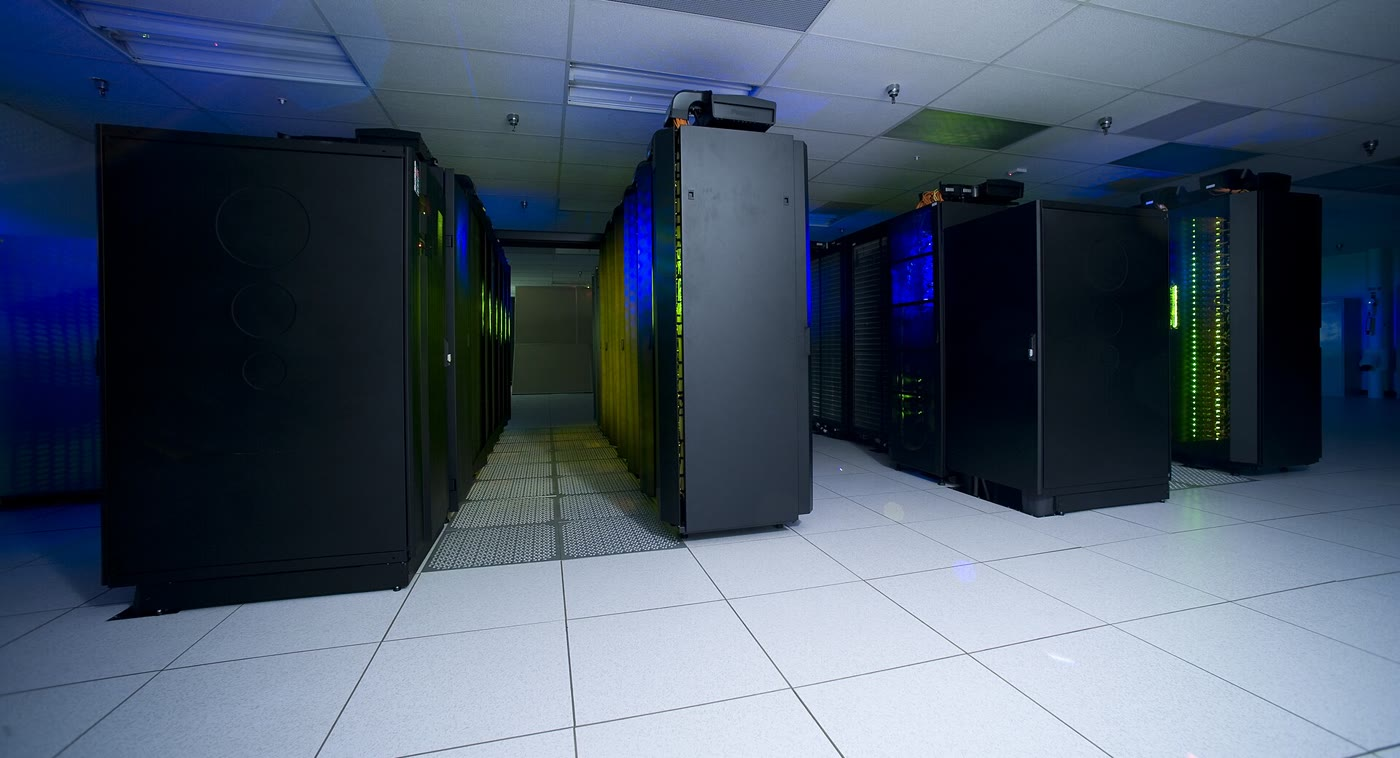
\includegraphics[width=0.7\linewidth]{images/book5/b3-nccs-supercomputer.jpg}

\par\smallskip{\small رفوف حاسوب فائق في مركز
\babelsublr{NASA Center for Climate Simulation}، في \babelsublr{Goddard Space Flight Center}، عام 2010 (\mbox{\textdir TLT NASA}، ملك عام).
تُحلّ المعادلات العددية للنموذج العالمي على حواسيب من هذا النوع
عالية الأداء.}\label{fig:b3:climate-models:supercomputer}
\end{omfigure}
% ledger: photo:b3-nccs, ar6ch1:esm

\section{تقييم النماذج}\label{sec:b3:climate-models:evaluation}

يُختبَر النموذج بمقارنته بالمناخ المرصود؛ والمشكلة أنّه
عُدِّل هو أيضًا وفقه. ولكلّ تمثيل بارامتري وسائط يُحدَّد مداها المقبول
بالفيزياء والرصد، ومع تجميع المكوّنات يُحسِّن النمذجون هذه الوسائط
حتى يطابق المناخ المحاكى مجموعةً من أهداف الضبط: المتوسط المناخي --- مثلًا،
درجة حرارة متوسطة قريبة من المرصودة تحت الإشعاع الشمسي الحالي --- والسمات الإقليمية،
أو اتجاهات الفترة التاريخية. عندئذٍ فقط يُطلَق النموذج
إلى مرحلة المقارنات
المتبادلة بين النماذج.
% ledger: ar6ch1:models, ar6ch1:parameterization, ar6ch1:large-ensembles

\begin{definition}[مشروع المقارنة بين النماذج]\label{def:b3:climate-models:cmip}
\emph{مشروع المقارنة بين النماذج}\index{مشروع المقارنة بين النماذج} هو مجموعة منسّقة
من التجارب --- بالتأثيرات الإشعاعية نفسها، والبروتوكولات نفسها، والمخرجات نفسها ---
تُجريها مجموعات نمذجة كثيرة بنماذجها الخاصة، كي تُقارَن النتائج.
ويجري \babelsublr{Coupled Model Intercomparison Project (CMIP)} على مراحل متتالية؛
وكانت مرحلته السادسة،
CMIP6، خطًّا رئيسيًا من أدلّة التقييم السادس.
\end{definition}

\begin{dated}{2021}
من بين 29 مجموعة نمذجة في CMIP6 أبلغت كيف ضبطت نماذجها، لم تضبط 23 منها
نماذجها على الاحترار المرصود في الفترة التاريخية، ولم تضبط 25 منها
حساسيتها المناخية ECS: فحساسية معظم النماذج خاصّيةٌ ناشئة، لا مُدخلٌ.
ومتوسطُ نماذج CMIP6 أعلى في ECS وTCR،
منه في نماذج المرحلة السابقة، وانتشارها أوسع من المدى الذي قيّمه التقرير؛
وفي بعض النماذج عُزي ذلك إلى التغذية الراجعة
للسحب في خطوط العرض المتوسطة والعالية. وتُعيد أشدّ النماذج حساسيةً
إنتاجَ الاحترار المرصود حديثًا والمناخات الماضية بصورة أضعف.
ولذلك لم يأخذ التقييم مدى ECS وTCR من النماذج مباشرةً،
بل من فهم عمليات التغذية الراجعة،
والسجلّ الآلي، والمناخات الماضية، والقيود الناشئة؛ ويعامل أشدّ النماذج حساسيةً بوصفها مرشدًا إلى نتائج
منخفضة الاحتمال وعالية الأثر (\emph{بدرجة ثقة عالية}).
\end{dated}
% ledger: ar6ch1:models, ar6ch7:cmip6-sensitivity

\begin{definition}[المجموعة الكبيرة؛ القيد الناشئ]\label{def:b3:climate-models:evaluation}
\emph{المجموعة الكبيرة}\index{المجموعة الكبيرة} هي مجموعةٌ من المحاكيات العددية
الكثيرة لنموذج واحد، بالتأثيرات الإشعاعية نفسها خلال الفترة نفسها، تختلف فقط
في حالاتها الابتدائية. و\emph{القيد الناشئ}\index{القيد الناشئ} علاقةٌ تُوجد
عبر مجموعة من النماذج المختلفة، بين كمّيةٍ قابلة للرصد في المناخ الحالي
وكمّيةٍ في المناخ المستقبلي، مثل ECS؛
فالقيمةُ المرصودة للأولى
تُضيّق مدى الثانية.
\end{definition}

المناخ فوضوي، فالفروق الصغيرة في الحالة الابتدائية تدفع أعضاءَ \omterm{def:b3:climate-models:evaluation}{المجموعة الكبيرة}
إلى مسارات مختلفة؛ فانتشار الأعضاء يقيس التباين الداخلي،
ومتوسطهم يقيس الاستجابة المفروضة. وقد دعمت مجموعاتٌ كبيرةٌ من عدّة نماذج التقييم.
ويحتاج \omterm{def:b3:climate-models:evaluation}{القيد الناشئ} إلى سببٍ فيزيائي.
وعبر بضعة عشرات من النماذج يمكن تجربة آلاف الكمّيات القابلة للرصد،
وسيترابط بعضها مع ECS بالصدفة؛ فأبقى التقييمُ تلك التي لها أساس فيزيائي،
كثيرٌ منها يتعلّق بالسحب في المناطق الاستوائية،
وحذّر من أنّ انحيازًا مشتركًا بين جميع نماذج المجموعة
يُبطل الطريقة.
% ledger: ar6ch1:large-ensembles, ar6ch7:emergent

\begin{inthelab}[مركز نمذجة مناخية]
\begin{minipage}[t]{0.55\linewidth}\vspace{0pt}
في مركز نمذجة مناخية، يكون النموذج برنامجًا يكتبه فريق ويصونه: الغلاف الجوي
والمحيط والجليد البحري واليابسة مكوّنات منفصلة، تتبادل الدفقات عند حدودها
عبر وحدة الاقتران. وقبل كل تشغيل تُقرأ التأثيرات الإشعاعية للتجربة ---
تراكيزُ غازات الدفيئة، والهباءات الجوية، واستخدامات الأراضي المنصوص عليها في البروتوكول.
يُقسَّم الكوكب إلى قطع تحسبها معالجات الحاسوب الفائق جنبًا إلى جنب،
ويتحوّل قرنٌ من المناخ المحاكى إلى أرشيف ضخم من الحقول.
ويعرض العلماء هذه الحقول على الشاشات،
ويقارنونها بإعادة التحليل وبسجلات الأقمار الصناعية،
ويرسلون المخرجات القياسية إلى أرشيف المقارنة المشتركة،
حيث تقارنها مجموعات أخرى بنماذجها الخاصة.
\end{minipage}\hfill
\begin{minipage}[t]{0.42\linewidth}\vspace{0pt}
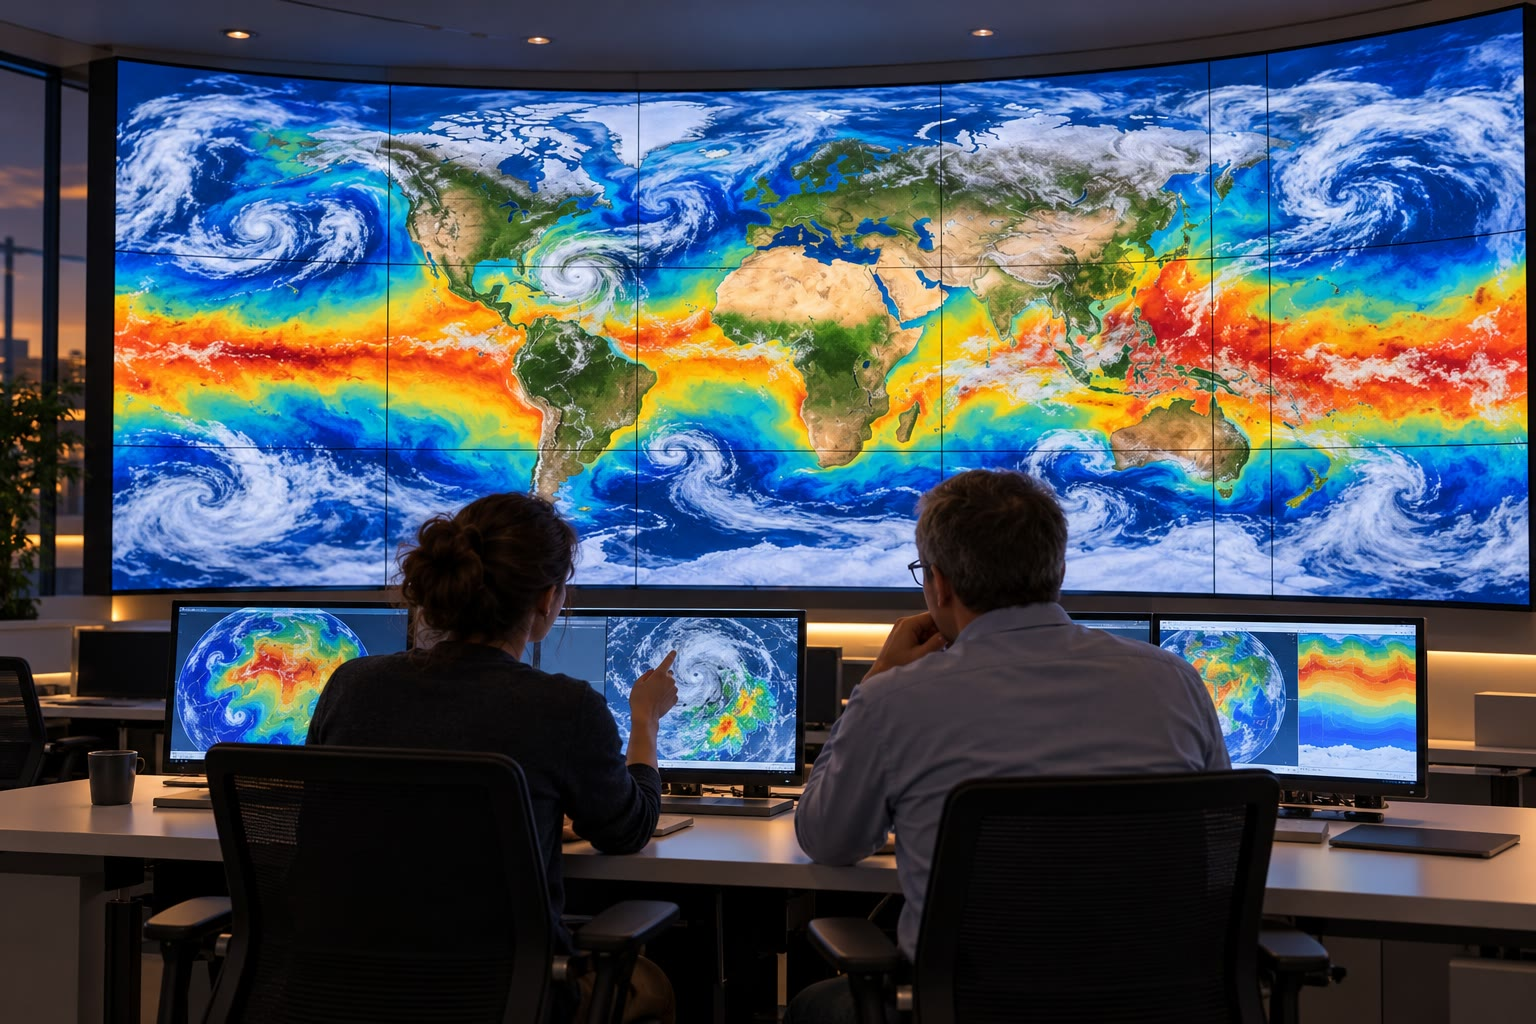
\includegraphics[width=\linewidth]{images/book5/ai/b3-model-centre.jpg}

{\scriptsize عالمان أمام جدار من الشاشات تعرض حقولًا عالمية
لتشغيل نموذج (رسم توضيحي مولَّد بالذكاء الاصطناعي).}
\end{minipage}
\end{inthelab}
% ledger: ar6ch1:esm, ar6ch1:models

\section{التمارين}

\begin{exercise}[$\star$]\label{exo:b3:climate-models:1}
قانون OLR عند بوديكو هو $I = a + bT - (a_1 + b_1T)n$، مع $a = 14.0$، $b =
0.14$، $a_1 = 3.0$، $b_1 = 0.10$، بوحدة \unit{kcal.cm^{-2}} لكل شهر، و$T$
بوحدة \unit{\celsius}. من أجل نسبة غيوم $n = 0.5$، احسب $A$ و$B$،
وحوّلهما إلى \unit{W/m^2} و\unit{W.m^{-2}.\celsius^{-1}}، مع أخذ الشهر
جزءًا من اثني عشر من سنة طولها 365.25 يومًا. ما قيمة OLR التي يعطيها القانون عند
\qty{15}{\celsius}؟
\end{exercise}
% ledger: budyko69:olr

\begin{exercise}[$\star$]\label{exo:b3:climate-models:2}
بفرض $Q = \qty{340}{W/m^2}$، و$A = \qty{211.9}{W/m^2}$، و$B =
\qty{1.816}{W.m^{-2}.\celsius^{-1}}$، احسب درجة حرارة التوازن
من أجل الألبيدو بقيمة 0.30 وبقيمة 0.31. بكم يبرّد هذا الكوكب ارتفاعُ
الألبيدو بمقدار 0.01؟
\end{exercise}

\begin{exercise}[$\star$]\label{exo:b3:climate-models:3}
احسب السعة الحرارية لكل متر مربع من طبقة مختلطة من مياه البحر
عمقها \qty{60}{m}، و$\rho = \qty{1025}{kg/m^3}$ و$c_p = \qty{3992}{J.kg^{-1}.K^{-1}}$،
بوحدة \unit{J.m^{-2}.K^{-1}} وبوحدة \unit{W.yr.m^{-2}.K^{-1}}. احسب
زمن الاستجابة حسب \cref{thm:b3:climate-models:response} من أجل $\lambda = -B =
\qty{-1.816}{W.m^{-2}.\celsius^{-1}}$ ومن أجل $\lambda =
\qty{-1.33}{W.m^{-2}.\celsius^{-1}}$.
\end{exercise}
% ledger: teos10:cp0

\begin{exercise}[$\star$]\label{exo:b3:climate-models:4}
بالنسبة إلى \omterm{def:b3:climate-models:ebm}{نموذج توازن الطاقة} ذي الطبقتين، حيث $\lambda = \qty{-1.33}{W.m^{-2}.\celsius^{-1}}$،
و$\gamma = \qty{0.62}{W.m^{-2}.\celsius^{-1}}$ و$F_{2\times} =
\qty{3.93}{W/m^2}$، احسب ECS، و TCR التقريبية $F_{2\times}/
(\gamma - \lambda)$، ثم نسبتهما.
\end{exercise}
% ledger: ar6sm7:two-layer, ipcc:erf-2xco2

\begin{exercise}[$\star\star$]\label{exo:b3:climate-models:5}
في النموذج صفري البعد الوارد في النص، خذ ثابت الشمس بقيمة
\qty{1340}{W/m^2}. أوجد التوازنات الثلاثة وميل التدفق الصافي $N'(T)$
عند كل منها، وأيّها مستقرّ؟
\end{exercise}

\begin{exercise}[$\star\star$]\label{exo:b3:climate-models:6}
انقل منحدر الألبيدو الوارد في النص: $\alpha = 0.62$ دون \qty{-20}{\celsius}،
و$0.30$ فوق \qty{0}{\celsius}، وخطيًّا فيما بينهما. أبقِ $A$ و$B$. عند أيّ
ثابت شمسي ينتهي الفرع الدافئ، وبكم في المئة يقلّ ذلك عن
\qty{1360}{W/m^2}؟ وعند أيّ ثابت شمسي تذوب الكرة الثلجية؟
ما الذي يحدّد حجم العتبة؟
\end{exercise}

\begin{exercise}[$\star\star$]\label{exo:b3:climate-models:7}
كوكب نموذجي بالمعاملات الواردة في النص موجود في حالة الكرة الثلجية.
(أ)~ما درجة حرارته عند ثابت الشمس الحالي؟ (ب)~مع إبقاء الشمس
كما هي، ما التأثير الإشعاعي $F$ الذي يرفع درجة حرارة الكرة الثلجية إلى
\qty{-10}{\celsius}؟ وكم مرّة يبلغ ذلك التأثير قيمة تأثير مضاعفة ثاني أكسيد الكربون،
أي \qty{3.93}{W/m^2}؟ (ج)~بعد زوال الجليد، أين يستقرّ
الكوكب إذا أُزيل التأثير الإشعاعي بعدئذٍ؟
\end{exercise}
% ledger: ipcc:erf-2xco2, hoffman17:hysteresis

\begin{exercise}[$\star\star$]\label{exo:b3:climate-models:8}
النموذج X، وهو نموذج مُتخيَّل ذو طبقتين، له $C = 7.0$ و$C_d =
\qty{90}{W.yr.m^{-2}.\celsius^{-1}}$، و$\gamma = 0.70$ و$\lambda =
\qty{-1.10}{W.m^{-2}.\celsius^{-1}}$. احسب مقياسَي الزمن للنموذج بدقّة
وبالتقريبات المذكورة في \cref{thm:b3:climate-models:two-layer}، الكسر
$a_f$، و ECS الخاصة به، و TCR التقريبية.
\end{exercise}

\begin{exercise}[$\star\star$]\label{exo:b3:climate-models:9}
في نموذج بوديكو الوارد في النص، $\bar T = \qty{12.81}{\celsius}$، $\beta =
\qty{3.74}{W.m^{-2}.\celsius^{-1}}$، وخطّ الجليد عند \ang{72}، و$s = 1.221$
عند خط الاستواء، و$0.506$ عند القطب، و$\alpha = 0.30$ و$0.62$.
احسب درجة الحرارة عند خط الاستواء وعند القطب، والحرارة $\beta(T - \bar T)$
التي يُزيلها النقل من كل
متر مربع هناك أو يجلبها إليه.
\end{exercise}

\begin{exercise}[$\star\star\star$]\label{exo:b3:climate-models:10}
كوكب خالٍ من الجليد ($\alpha = 0.30$ في كل مكان) له النقل الانتشاري
$D = -\mathcal D\,\partial_x[(1 - x^2)\partial_xT]$
والإشماس $s(x) = 1 + s_2P_2(x)$، $P_2 = (3x^2 - 1)/2$. (أ)~أثبت أنّ
$\partial_x[(1 - x^2)\partial_xP_2] = -6P_2$. (ب)~أثبت أنّ $T = T_0 +
T_2P_2(x)$ حلٌّ مستقرّ، مع $T_0 = (Q(1 - \alpha) - A)/B$
و$T_2 = Qs_2(1 - \alpha)/(B + 6\mathcal D)$. (ج)~إشماس إعادة التحليل
يعطي $s_2 = \num{-0.476}$. بدون النقل، ما فرق درجة الحرارة
بين خط الاستواء والقطب؟ (د)~أيّ $\mathcal D$ يعطي الفرق المرصود،
\qty{55.3}{\celsius}؟
\end{exercise}
% ledger: data:b3-ncep, data:b5-ncep-air

\begin{exercise}[$\star\star\star$]\label{exo:b3:climate-models:11}
(أ)~اكتب المعادلة التربيعية في \cref{thm:b3:climate-models:two-layer} على الصورة $r^2 -
\Sigma r + \Pi = 0$، وأثبت أنّه إذا كان $4\Pi \ll \Sigma^2$، فإنّ جذريها
قريبان من $\Sigma$ و$\Pi/\Sigma$. (ب)~بالنسبة إلى قوة $F = kt$ المتزايدة خطيًّا،
أثبت أنّه متى كان $t \gg \tau_f$، وطالما بقي $T_d$ صغيرًا،
فإنّ $T \approx kt/(\gamma - \lambda)$؛ استنتج TCR التقريبية. (ج)~تحقّق
من الأرقام الواردة في النص: $\Sigma$، و$\Pi$، ومقياسا الزمن،
والنسبة $4\Pi/\Sigma^2$.
\end{exercise}
% ledger: ar6sm7:two-layer

\begin{exercise}[$\star\star\star$]\label{exo:b3:climate-models:12}
مجموعة مُتخيَّلة من ثمانية نماذج تعطي المتغيّر القابل للرصد $X$ للمناخ
الحالي، و ECS الخاصة بها:
\begin{center}
\begin{tabular}{l*{8}{c}}
\hline
$X$ & 0.2 & 0.5 & 0.6 & 0.8 & 1.0 & 1.1 & 1.3 & 1.5\\
\mbox{\textdir TLT ECS (\unit{\celsius})} & 2.3 & 2.7 & 3.1 & 3.2 & 3.8 & 3.9 & 4.4 & 4.6\\
\hline
\end{tabular}
\end{center}
(أ)~احسب متوسط ECS والانحراف المعياري لها في
المجموعة. (ب)~أجرِ ملاءمة \mbox{\textdir TLT ECS $= a + bX$} بطريقة المربعات الصغرى، واحسب الترابط
والانحراف المعياري للبواقي. (ج)~المتغيّر المرصود $X$ هو $0.7
\pm 0.1$. ما ECS التي يعطيها \omterm{def:b3:climate-models:evaluation}{القيد الناشئ}، وبأيّ انتشار؟
(د)~ما الذي يدعوك إلى عدم الثقة بهذا \omterm{def:b3:climate-models:evaluation}{القيد الناشئ}؟
\end{exercise}
% ledger: ar6ch7:emergent

\section{مسألة: إلى أي مدى نقترب من كرة الثلج؟}

\begin{problem}[{مسألة نهاية الأسبوع --- الاتزان والاستقرار
وعتبة التجمّد لكوكب نموذجي}]
\label{pb:b3:climate-models:1}
يملك كوكب نموذجي ثابت الشمس الحالي $S_0 = \qty{1360}{W/m^2}$
وقانون الإشعاع طويل الموجة الخارج $A + BT$ مع $A = \qty{211.9}{W/m^2}$ و$B =
\qty{1.816}{W.m^{-2}.\celsius^{-1}}$. ألبيدوه 0.62 دون \qty{-10}{\celsius}،
و0.30 فوق \qty{+10}{\celsius}، ويتغيّر خطيًّا بينهما،
وسعته الحرارية السطحية $C = \qty{8.1}{W.yr.m^{-2}.\celsius^{-1}}$. خذ
$\sigma = \qty{5.670e-8}{W.m^{-2}.K^{-4}}$.

\medskip\noindent\textbf{الجزء الأول --- الكوكب في حالة اتزان.}
\begin{enumerate}
\item احسب متوسط ضوء الشمس $Q_0$ لكل متر مربّع من الكوكب،
  واشرح العامل.
\item احسب ضوء الشمس الممتص عند ألبيدو 0.30، والإشعاع طويل الموجة الخارج عند
  \qty{15}{\celsius}.
\item احسب الاتزان الدافئ.
\item احسب اتزان كرة الثلج، وتحقّق من أنّه يقع على الفرع
  الجليدي.
\item احسب الاتزان الثالث، على منحدر الألبيدو.
\item احسب درجة حرارة الانبعاث التي تُعيد ضوء الشمس الممتص إلى الفضاء
  بوصفه جسمًا أسود، وقارنها بالاتزان الدافئ.
\end{enumerate}

\medskip\noindent\textbf{الجزء الثاني --- الاستقرار والزمن.}
\begin{enumerate}[resume]
\item احسب ميل الدفق الصافي $N'(T)$ عند كلّ اتزان، وبيّن
  أيّها مستقرّ.
\item ينمو انحراف صغير عن الاتزان الأوسط وفق $\mathrm
  e^{t/\tau}$. احسب $\tau$.
\item احسب زمن الاستجابة للاتزان الدافئ.
\item تأثير إشعاعي مقداره \qty{3.93}{W/m^2}، وهو تأثير مضاعفة ثاني أكسيد الكربون،
  يُشغَّل. احسب الاحترار عند الاتزان، وقارنه بقيمة
  ECS المقدّرة للمناخ الحقيقي.
\item كم يستغرق النموذج لبلوغ \qty{95}{\percent} من
  الاحترار؟ لماذا يستغرق المناخ الحقيقي وقتًا أطول؟
\end{enumerate}

\medskip\noindent\textbf{الجزء الثالث --- \omterm{def:b3:climate-models:multiple-equilibria}{التشعّب السرجي العقدي}.}
\begin{enumerate}[resume]
\item مع خفوت الشمس، عند أيّ درجة حرارة يلتقي الاتزان الدافئ
  بالاتزان الأوسط؟ احسب $Q$ عندها.
\item احسب ثابت الشمس عند التشعّب، ومقدار الانخفاض عن
  اليوم بالنسبة المئوية.
\item أسفل التشعّب مباشرةً، إلى أين يتجه المناخ؟ احسب درجة حرارته.
\item احسب ثابت الشمس الذي تذوب عنده كرة الثلج، والارتفاع
  عن اليوم بالنسبة المئوية.
\item ارسم الحلقة التي تتبعها درجة الحرارة عندما يُخفَّض $S_0$
  دون التشعّب، ثم يُعاد إلى \qty{1360}{W/m^2}.
\end{enumerate}

\medskip\noindent\textbf{الجزء الرابع --- خط الجليد.} اعتمد للكوكب
نموذج بوديكو الخطي العرض، مع $\beta = \qty{3.739}{W.m^{-2}.\celsius^{-1}}$،
وألبيدو الجليد 0.62 باتجاه القطب من خط الجليد، و0.30 باتجاه خط الاستواء، و0.50 عند
الحافة، وضوء الشمس الوارد من إعادة التحليل:
\begin{center}
\begin{tabular}{lccccccc}
\hline
خط العرض & \ang{0} & \ang{30} & \ang{40} & \ang{47.5} & \ang{55} & \ang{60} & \ang{72}\\
$s(x_s)$ & 1.2211 & 1.0730 & 0.9647 & 0.8688 & 0.7650 & 0.6947 & 0.5643\\
$F(x_s)$ & 0 & 0.5865 & 0.7324 & 0.8192 & 0.8863 & 0.9205 & 0.9738\\
\hline
\end{tabular}
\end{center}
\begin{enumerate}[resume]
\item عندما يكون خط الجليد عند \ang{72}، احسب متوسط الألبيدو $\bar\alpha$
  ومتوسط درجة الحرارة $\bar T$.
\item احسب درجة الحرارة الحرجة $T_c$ التي تضع الحافة عند
  \ang{72} اليوم، وقارنها بإعادة التحليل، \qty{-15.8}{\celsius}.
\item احسب بسط $Q(x_s)$ في \cref{prop:b3:climate-models:iceline}
  ونسبة $\beta/B$.
\item احسب $Q(x_s)/Q_0$ لخط الجليد عند \ang{30}، \ang{40}،
  \ang{47.5}، \ang{55} و\ang{60}.
\item أين يقع الحدّ الأدنى لهذه القيم؟ أيّ خطوط الجليد مستقرّة؟
\item مع شمس اليوم، أيّ خط جليد آخر يسمح به النموذج، وهل هو
  مستقرّ؟ وهل كرة الثلج ممكنة اليوم؟ (استخدم العمود \ang{0}.)
\item قارن عتبة النموذج الخطي العرض بعتبة الجزء الثالث
  وبعتبة بوديكو البالغة \qty{1.6}{\percent}، وقارن خط عرض الجليد عند العتبة
  بخط عرضه \ang{50}.
\item أعطِ، برقمين معنويين، مقدار انخفاض ثابت الشمس
  بالنسبة المئوية الذي يُغطّي الكوكب النموذجي بالجليد.
\end{enumerate}
\end{problem}
% ledger: nasa:solar-mean, data:b5-ncep-air, data:b3-ncep, budyko69:transport, budyko69:albedo, budyko69:threshold, ipcc:ecs, const:sigma
